\section{Scientific Computing.}

\subsection{Sarrera.}

Gaur-egun, orohar konputagailuak (superkonputagailu, portatila,...) paraleloak dira. 1986-2002 urteen artean,  prozesadore bakarreko konputagailuen eraginkortasuna hobetuz joan zen, txipean transistore dentsitatea handitzen zen heinean   baina teknologi-garapena muga fisikoetara iritsita, bide honetatik konputagailuen abiadura hobetzea ezinezkoa bilakatu zen. Horrela, 2005.urtetik aurrera fabrikatzaileek konputagailuen gaitasuna hobetzeko, txipan prozesadore bat baino gehiago erabiltzea erabaki zuten.      

\paragraph*{Moore's Law (1965)}. Processor speed doubles every 18 months.

\paragraph*{Moore's Law Reinterpreter}. Number of cores per chip can double every two years.

\begin{figure}[h]
\centerline{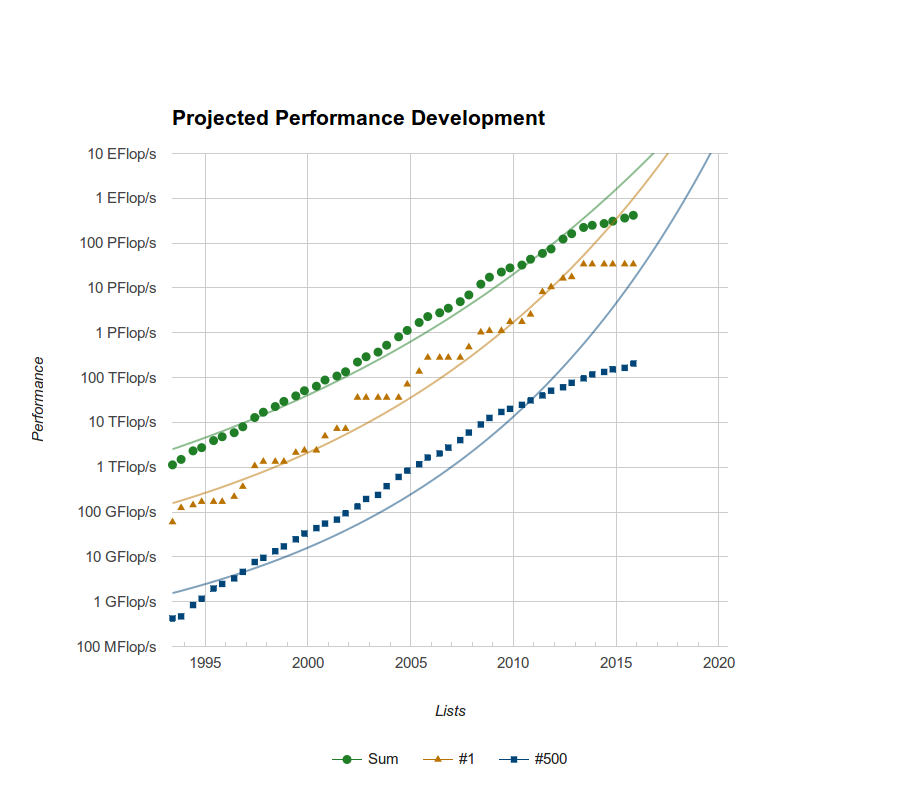
\includegraphics[width=12cm, height=8cm] {PerformanceDevelopment}}
\caption{www.top500.org, Top: total computing power of top 500 computers. Middle: 1 computer. Bottom: 500 computer.}
\label{fig:61}
\end{figure} 

\paragraph*{} Konputagailuen eredu aldaketa honen ondorioz, algoritmo azkarrak garatzeko kodearen paralelizazio gaitasunari heldu behar zaio. Beraz programazio paralelo teknikak inplementatzeko, beharrezko da prozesadore berrien hardware arkitekturak nahiz software ingurune berriak ulertzea. Gaia nahiko konplexua izanik, ikuspegi orokorra eman ondoren, gure inplementazioan erabilitako hardware arkitektura eta software teknika zehatzak azalduko ditugu. Memoria-konpartitutako sistemak eta OpenMP programazio eredua deskribatuko dugu.

\paragraph*{}Bi dira, algoritmo azkarrak disenatzeko erronkak: 
\begin{enumerate}
\item Paralelizatzeko pisuko lana identifikatzea.
\item Memoria eta prozesadorearen arteko datu mugimendua gutxitzea. 
\end{enumerate}

\paragraph*{}Bestalde, inplementazio berrien garapenean optimizatutako liburutegiak erabiltzea komeni da. Horien artean, LAPACK eta BLAS algebra linealeko liburutegiak erabilgarriak izan zaizkigu. Liburutegi hauen gaineko azalpenak emango ditugu.

\subsection{Parallel Hardware.}

\subsubsection*{\textbf{Zein azkarrak dira konputagailuak?}}

\paragraph*{}Gaur egungo prozesadoreen abiadura Gigahertzioetan neurtzen da. 

\begin{itemize}
\item Kilo = mila ($10^3$).
\item Mega = milioi ($10^6$).
\item Giga = bilioi ($10^9$).
\item Tera = trilioi ($10^{12}$).
\item Peta = $10^{15}$.
\item Exa = $10^{18}$. 
\end{itemize}

\paragraph*{} Hertzioak "makina zikloak segunduko" esan nahi du. Koma-higikorrezko  eragiketa bat egiteko ($\oplus,\ominus,\otimes,\oslash$) ziklo gutxi batzuk behar dira. Honek esan nahi du, $1$GHz-ko prozesagailu batek,
$>100.000.000$ koma-higikorrezko eragiketa segunduko egiten dituela ($>100$ Megaflops).

\paragraph*{\textbf{Adibidea}}. 
$C=AB$ matrize-matrize biderketa.

\paragraph*{}Demagun $A,B$ eta $C \ (n \times n)$ dimentsioko matrizeak.

\begin{equation*}
c_{ij}=\sum\limits_{i,j=1}^{n} a_{ij}*b_{ji}
\end{equation*}

\paragraph*{} $c_{ij}$ gai bakoitza kalkulatzeko $n$ biderketa eta ($n-1$) batura egin behar ditugu.

$C$ matrizeak $n^2$ osagaia ditu $\Rightarrow$ $O(n^3)$ koma-higikorrezko ariketak.

$n=1000 \ \Rightarrow \ n^3=10^{12}$

$>1000$ segundu $1$GHz prozesagailuan.

\paragraph*{} Zientzia konputazioaren eraginkortasuna neurtzeko, koma-higikorrezko eragiketa kopurua (flops) erabiltzen zen. Problema handia denean, datuen mugimendua koma-higikorrezko eragiketak baino garestiagoa da, eta beraz eraginkortasuna aztertzeko koma-higikorrezko eragiketa kopurua neurtzea okerra izan daiteke. Kodearen exekuzioa azkartzeko derrigorrezkoa da konputagailuan datuen mugimendua minimizatzea.

\subsubsection*{\textbf{Memoria Hierarkia.}}

\paragraph*{}Lehenik, konputagailuan dauden memoria mota ezberdinen hierarkia azalduko dugu. 

\begin{figure}[h]
\centerline{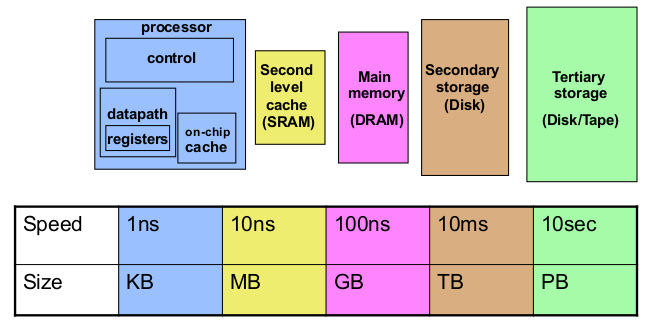
\includegraphics[width=10cm, height=4cm] {MemoryHierarchy}}
\caption{Memoria hierarkia.}
\label{fig:three}
\end{figure} 

\paragraph*{} CPU-k koma-higikorrezko eragiketak egiten ditu: datuak erregistroetatik irakurri, eragiketa egin eta emaitza erregistroetan idazten ditu. Memoria nagusia eta erregistroen artean, 2 edo 3 mailako Cache memoria dugu: lehen Cache memoria (L1) txikiena eta azkarrena da, eta beste mailak (L2,L3,...), handiagoak eta motelagoak. Memoria nagusian, exekutatzen diren programak eta datuak gordetzen dira ($1-4$ GB artekoa). Azkenik, disko gogorrean konputagailuko datu (argazki, bideo,...) eta erabilgarri ditugun programa guztiak gordetzen dira.  
   
\paragraph*{} Cache memorian, programak hurrengo unean behar dituen datuak gertu dauden printzipioaren arabera gordetzen da informazioa. Cache memoria blokeka (line) egituratuta dago eta bloke bakoitza $64$ edo $128$ bytez ($8$ edo $16$ double zenbaki) osatuta dago. 

\paragraph*{\textbf{Adibidea}}. Badakigunez, C-lengoaian matrizeak lerroka gordetzen dira. Beheko adibidean,  matrizearen lehen osagaia $a(1,1)$ behar dugunean, memoria nagusitik Cachera osagai honetaz gain jarraiko 16 osagaiak ekarriko dira ($a(1,1),a(1,2),\dots,a(1,16)$). Honela, hurrengo $15$ batura egiteko behar ditugun datuak Cachean eskuara izango ditugu memoria irakurketa berririk egin gabe. 

\begin{algorithm}[h]
 \BlankLine
  $int \ n$\;
  $double \ a[n][n]$\;
  \BlankLine
  $sum=0$\;
  \For{$i\leftarrow 1$ \KwTo $n$}
  {
   \BlankLine
    \For{$j\leftarrow 1$ \KwTo $m$}
   {
    \BlankLine 
    $sum+=a(i,j)$\;
   }
 }
 \caption{Main Algorithm}
\end{algorithm} 

\begin{equation*}
a=\left(\begin{array}{ccccc}
  1    & 2    & 3    & \dots & 1000 \\
  1001 & 1002 & 1003 &\dots & 2000 \\
  2001 & 2002 & 2003 &\dots & 2000 \\
  \dots & \dots & \dots & \dots & \dots \\
  9001 & 9002 & 9003 &\dots & 10000 \\
  \end{array}\right).  
\end{equation*}

\paragraph*{}CPUk datu bat behar duenean, memoria hierarkian zehar bilatuko du: lehenik $L1$ cachean, ondoren $L2$ cachean,...eta hauetan ez badago, memoria nagusira joko du. Memoria nagusi eta cache memoria arteko irakurketa eta idazketa guzti hauetan,  informazio konsistentzia mantentzeko hainbat arau aurrera ematen dira.  

\subsubsection*{\textbf{Hardware.}}

MIMD (Multiple instruction, multiple data) sistemak, guztiz independienteak diren prozesadore multzoak osatzen dituzte. Bi dira MIMD sistema nagusiak: memoria konpartitutako eta memoria distribuitutako sistemak. Memoria konpartitutako sistemetan, prozesadore guztiek memoria osoa konpartitzen dute eta inplizituki konpartitutako datuen atzipenaren bidez komunikatzen dira. Memoria distribuitutako sistemetan aldiz, prozesadore bakoitzak bere memoria pribatua du eta explizituki bidalitako mezuen bidez komunikatzen dira.

\paragraph*{} Hirugarren hardware arkitektura ere aipatuko dugu, general purpose GPU computing (Graphical Processor Unit).
Jokuen eta animazio industriak, grafiko oso azkarrak beharrak biltzatuta  sortutako teknologia da. Oinarrian, imaginak oantailaratzeko prozesagailu asko paraleloan lan egiten dute. Azken hamarkadan, GPU unitate hauek zientzia konputaziora zabaldu dira.  

\begin{figure}[h]
\centerline{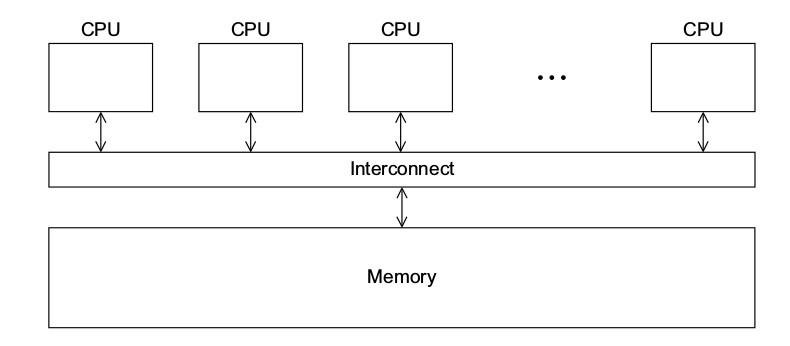
\includegraphics[width=12cm, height=4cm] {SharedMemorySystem}}
\caption{Shared Memory System.}
\label{fig:61}
\end{figure}  

\begin{figure}[h]
\centerline{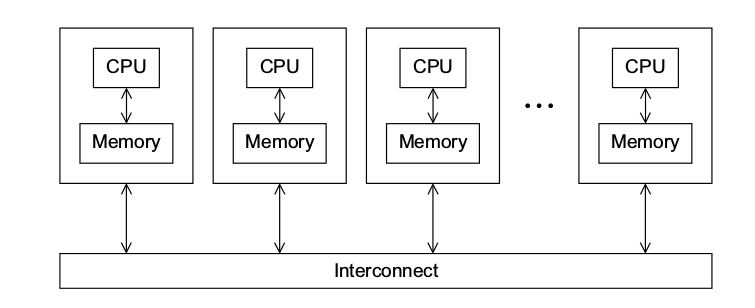
\includegraphics[width=12cm, height=4cm] {DistribuitedMemorySystem}}
\caption{Distribuited Memory System.}
\label{fig:61}
\end{figure}  

\paragraph*{\textbf{Shared-memory systems}}. Multicore bat edo gehiagoz osatutako sistema dugu. Multicore prozesadore bakoitzak txipean CPU bat baino gehiago ditu. Normalean CPU bakoitzak $L1$ bere cache memoria du. Aipatzeko da, era honetako sistemetan prozesadore kopurua ezin dela nahi adina handitu eta mugatua dela (normalean $\leq 32$ ).

 \begin{figure}[h]
 \centerline{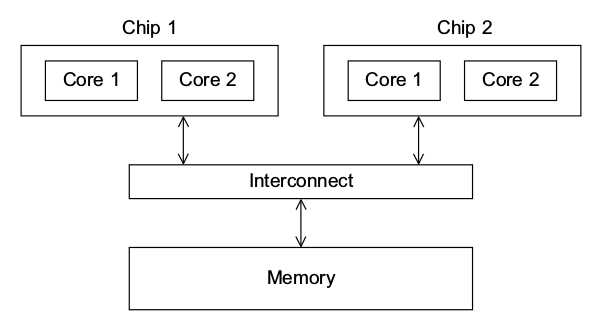
\includegraphics[width=12cm, height=4cm] {SharedMemorySystemUMA}}
 \caption{Shared Memory System (UMA).}
 \label{fig:61}
 \end{figure}  

\subsubsection*{\textbf{Sofwarea.}}

C-lengoaia programazio paraleloan erabiltzeko, lengoiaren bi extensio dira nagusienak: bata memori-distribuitutako sistemetarako diseinatuta  MPI (Message-Passing Inteface) eta bestea, memoria-konpartitutako sistemetarako diseinutakoa OpenMP (Open Specifications for MultiProcessing). MPI datu moten definizio, funtzio eta makroen liburegia da. OpenMP liburutegia bat  eta C konpiladorearen aldaketa batzuk. OpenMP erabili dugu gure inplementaziorako eta jarraian honi buruzko idei nagusienak emango ditugu.

\paragraph*{\textbf{OpenMP}}. Memoria konpartitutako programazio paraleloaren estandarra dugu. 
Programazioan paralelizazio kontrola, "fork-join" modeloa jarraituz egiten da.

\begin{enumerate}
\item OpenMP programen hasieran prozesu bakarra dago, hari (thread) nagusia. 
\item FORK: hari nagusiak hari talde paraleloa sortzen du.
\item JOIN: hariak kode paraleloa bukatzen dutenean, behin sinkronizatuta amaitzen dute eta hari nagusiak bakarrik jarraitzen du.
\end{enumerate}

 \begin{figure}[h]
 \centerline{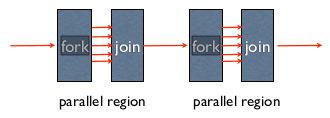
\includegraphics[width=10cm, height=3cm] {ForkJoin}}
 \caption{Fork-Join.}
 \label{fig:61}
 \end{figure}  

Aldagai batean (threadcount) paralelizazioan zenbat hari erabili adierazten da eta ohikoa izaten da hari bat prozesadore bakoitzeko sortzea.  Konpilazio direktiben bidez,  paralelizazioa nola exekutatu behar den zehazten zaio.

\paragraph*{\textbf{Adibidea}}.

\begin{lstlisting}
#    pragma omp parallel for num_threads(thread_count) 
     for (i = 0; i<n; i++)
     {
       ! Aginduak 
     }
\end{lstlisting}

\subsection{Software liburutegiak.}

Matematika bi software errekurtso nagusienak aipatuko ditugu; BLAS (Basic Linear Algebra Subroutines) eta LAPACK (Linear Algebra Package). Kalitate handiko software orokorrak dira eta hauek erabiltzea abantaila asko ditu: 

\begin{enumerate}
\item Garapen berriak egiteko denbora aurrezten du. 
\item Problema askotan ondo probatutako softwareak dira.
\item Konplexutasun handikoak dira, modu seguruan eta azkarrean exekutatzeko disenatu direlako. 
\end{enumerate}

Konputagailu hardware bakoitzerako optimizatutako bertsioak daude. Inplementazioa Fortranen egina dago eta datu-motei dagokionez:

\begin{enumerate}
\item S: float ($32$ bit).
\item D: double ($64$ bit).
\item C: complex.
\item Z: complex double.
\end{enumerate}   

\subsubsection*{\textbf{BLAS}}.

BLAS liburutegian, bektore eta matrizeen arteko funtzio estandarrak inplementatuta daude. Hiru mailetan banatuta dago: 

\begin{enumerate}
\item BLAS-1: bektore-bektore eragiketak.

 Adibidez: $y=\alpha*x+y$ , $2n$ flop eta $3n$ irakurketa/idazketa.
 
 Konputazio intentsitatea: $\frac{2n}{3n}=\frac{2}{3}$. 

\item BLAS-2: matrize-bektore eragiketak.

 Adibidez: $y=\alpha*A*x+\beta*x$, $O(n^2)$ flop eta $O(n^2)$ irakurketa/idazketa.
 
 Konputazio intentsitatea: $\approx \frac{2n^2}{n^2}=2$. 
 
\item BLAS-3: matrize-matrize eragiketak.

 Adibidez: $C=\alpha*A*B+\beta*C$, $O(n^3)$ flop eta $O(n^2)$ irakurketa/idazketa.
 
 Konputazio intentsitatea: $\approx \frac{2n^3}{4n^2}=\frac{n}{2}$. 

\end{enumerate}

Azpimarratu, BLAS-1 eta BLAS-2 funtzioen konputazio intetsitatea txikia dela eta beraz, datuen komunikazioa nagusia dela. BLAS-3 aldiz, konputazio intentsitatea handiagoa da eta eazugarri honi esker, konputagailuaren konputazio gaitasuna ondo aprobetxatu ahal izango da.

\begin{figure}[h]
\centerline{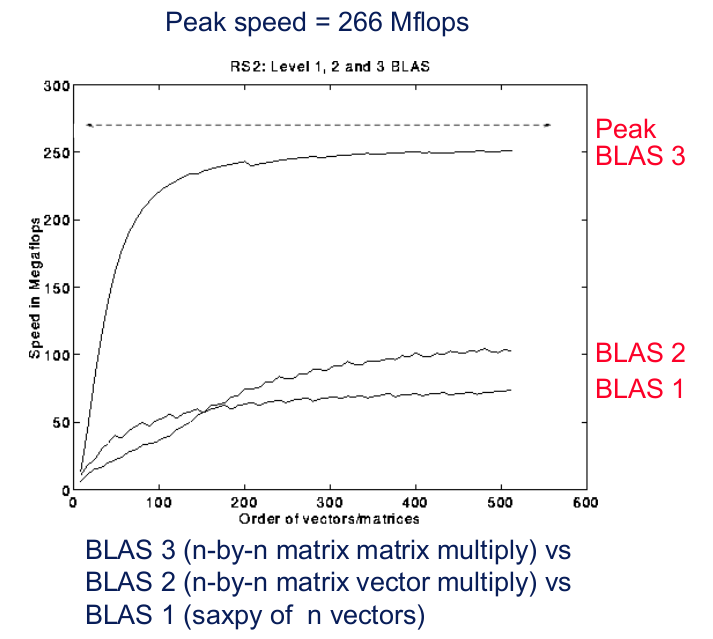
\includegraphics[width=12cm, height=8cm] {BLASSpeed}}
\caption{BLAS speeds.}
\label{fig:61}
\end{figure}    

Fabrikatzaile bakoitzak optimizatutako BLAS liburutegiak (AMD ACML,Intel MKL) dituzte eta beraz, multi-threaded dira.
Beste aukera bat, optimizatutako BLAS instalazioa ATLAS (Automatically Tuned Linear Algebra Software) bidez egitea.    

\subsubsection*{\textbf{LAPACK}}.

Zenbakizko algebra linealaren liburutegia da.

\begin{enumerate}
\item Sistema linealak: $AX=b$.
\item Least Square: choose $x$ to minimize $\|Ax-b\|$.
\item Eigenvalues.
\item Balio singularren deskonposaketa (SVD).
\end{enumerate}

Posible den guztietan, BLAS-3 funtzioetan oinarritzen da.


\subsection{Laburpena.}

Algoritmo bat inplementatzen dugunean kontutan hartu beharrekoa:

\begin{enumerate}

\item Lerro edo zutabe araberako iterazioak exekuzio denboran eragin handia du.

\item Kodea garbia eta ulergarria mantendu behar da.

\item Badaude kodearen exekuzio denboraren analisia egiteko tresnak (adibidez gprof). Algoritmoaren funtzio bakoitzaren exekuzio denborari buruzko informazio erabilgarria lortuko dugu. Zenbait gauza modu sinplean azkartu daitezke baina zenbait beste gauza azkartzeko esfuertzu handia eskatu dezake.

\item Optimizatutako beste hainbat kode erabiltzea komenigarria da. LAPACK aljebra lineal paketea Fortran eta C-lengoaitetatik deitu daiteke. Eraberean, LAPACKek BLAS subrutinak erabiltzen ditu.  Subrutinak hauek matrizen arteko biderketak, "inner product", ... BLAS konputagailu arkitektura ezberdinetarako optimizatutako bertsioak daude.
 


\end{enumerate}

